\section{Le contexte}
\paragraph{}
At the time of working on this project, I've spent 5 semesters as a student at Faculty of Computer Science, Iași, and the last (current) one as an \href{https://ec.europa.eu/programmes/erasmus-plus/about_en}{Erasmus} student, at Université de Lille.
As fate has it, the \href{https://en.wikipedia.org/wiki/2019–20_coronavirus_pandemic}{COVID-19} outbreak is currently forcing us into at least 2 weeks of self-isolation, so what better opportunity to spend quality time working on this?
\paragraph{}
This is a double purposed project.
As an Erasmus student, I will have developed this project for the \href{https://www.fil.univ-lille1.fr/portail/index.php?dipl=MInfo&sem=S8&ue=PJI&label=Présentation}{``Projet Individuel'' course}, having a final soutenance at the end of May, 2020.
After having finished the Erasmus programme, the project will have been used as my thesis to obtain a Bachelor's Degree, at Faculty of Computer Science, Iași.

\section{L'idée}
\paragraph{}
The base idea is to have a software application that will track the user's face, with the purpose of moving the cursor position in real time.
For this, we will make use of a webcam to get image input.
Further, based on the image, we will try to calculate where the user is looking and finally move the mouse cursor accordingly.
\begin{figure}[H]
    \centering
    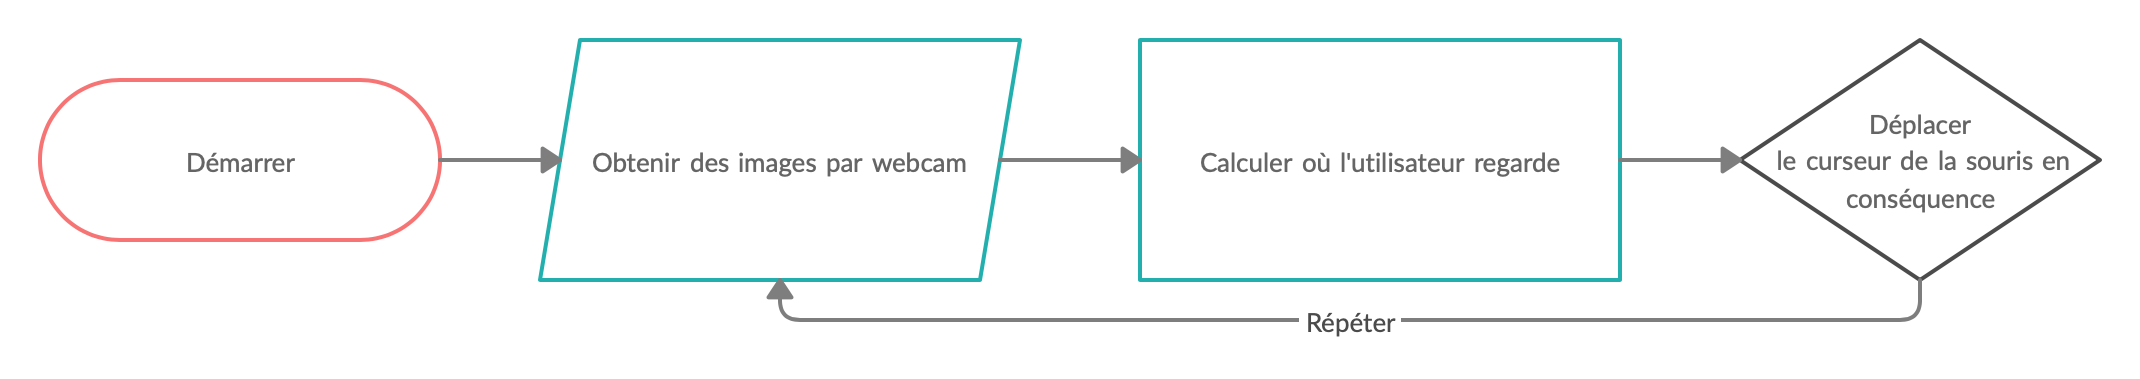
\includegraphics[width=\textwidth]{app_idea.png}
    \caption{Procédure générale}
\end{figure}

\section{Motivation}
\paragraph{}
When it came to deciding what project I wanted to work on, I took into account 2 key factors: my future professional career and the project's usability.
I wanted to work on something that would fuel my interest in Artifficial Intelligence and that would give me a chance to apply the research I will be making into this field.
Furthermore, I also wanted to have a practical approach towards this project and make something that will be useful for people.
\paragraph{}
Looking back in time, people have always worked on making technology accessible to as many people as possible.
Whether we're talking about the Braille system, helping blind people read and write, screen readers or intelligent assistants (Siri, Bixby etc.), accessibility is a key factor in making sure that people benefit from the advantages of technology.
Therefore, I'd feel a certain peace of mind knowing that I too worked on a project that could potentially help disabled people – and not only them – use the computer without the use of hands.
\paragraph{}
As for Artifficial Intelligence, it is needless to emphasize it's contemporany importance.
From medical applicability, autonomous driving and flying, smart farming and agriculture to having smart fridges that tell you when you're running out of milk, Artifficial Intelligence is widespread and it's growth isn't going to stop anytime soon.
For me, this is another reason to study it and get to understand it better, since it is being integrated in our everyday lives.
% As a bonus, I'll have the chance of using some of the knowledge I've gathered as a student throughout the time.
% to individually work on a project that will showcase my software development skills, but also the abilities of practical knowledge applying and researching on certain topics.

\section{Le but}
\subsection{Objectifs essentiels}
\paragraph{}
One of the first objectives I'll try to meet is approximately knowing where the user is looking only using the user's eyes.
For example, a good start would be to know which portion of the screen the user is focusing on.
Based on the grid below, if the user looks at square number $i$, then we will move the mouse cursor in the center of that square.
\begin{figure}[H]
    \centering
    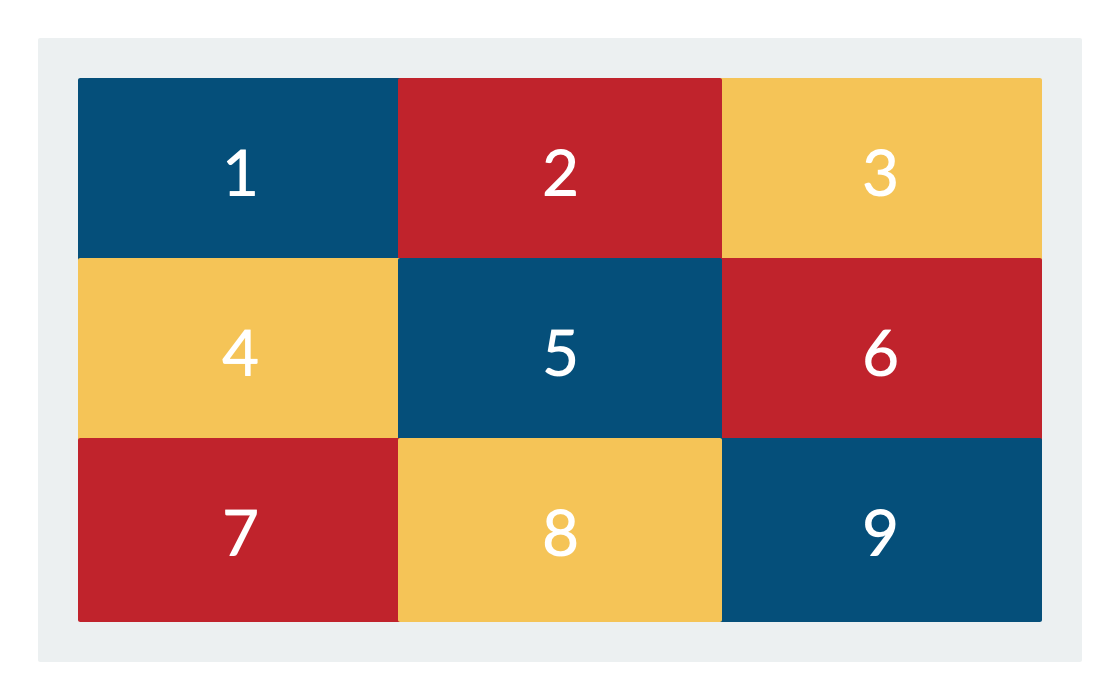
\includegraphics[width=\textwidth]{grid_3x3.png}
    \caption{3x3 grid}
\end{figure}

\paragraph{}
Secondly, I will try to simulate the click functions as follows: if the user closes his left eye for a certain amount of time, then we will interpret that as a left click.
The same will be done for the right click, using the right eye.

\paragraph{}
As some general guidelines, I will try to develop the application in order for it to be easily maintanable.
I'll also focus on concepts I have learned throughout university: clean code, OOP principles, SOLID principles, cohesion etc.
Also, a good requirement would be to make the application cross-platform.

\subsection{Objectifs préférables}
\paragraph{}
To go a little further, if predicting the squares goes well, we can try to predict the exact location of the cursor.
That means we'll move the mouse cursor exactly where we think the user will be looking.

\paragraph{}
Having more information about the user could help our calculations.
For that, I will also try to look into how I can use other parts of the face to improve the calculations: for example, the nose position.
The image below represents some facial landmarks we will use for our calculations: points $[37, 48]$ are for eyes and $[28, 36]$ for the nose.
\begin{figure}[H]
    \centering
    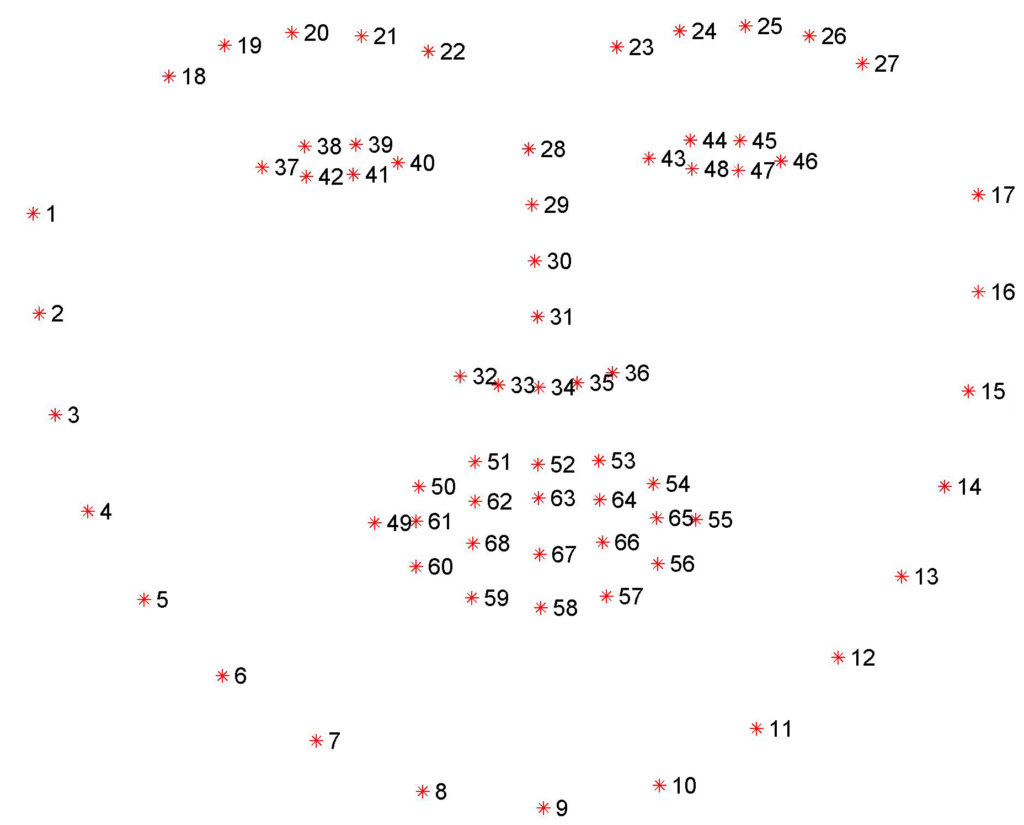
\includegraphics[width=\textwidth/2 - 10pt]{facial_landmarks_1.jpg}
    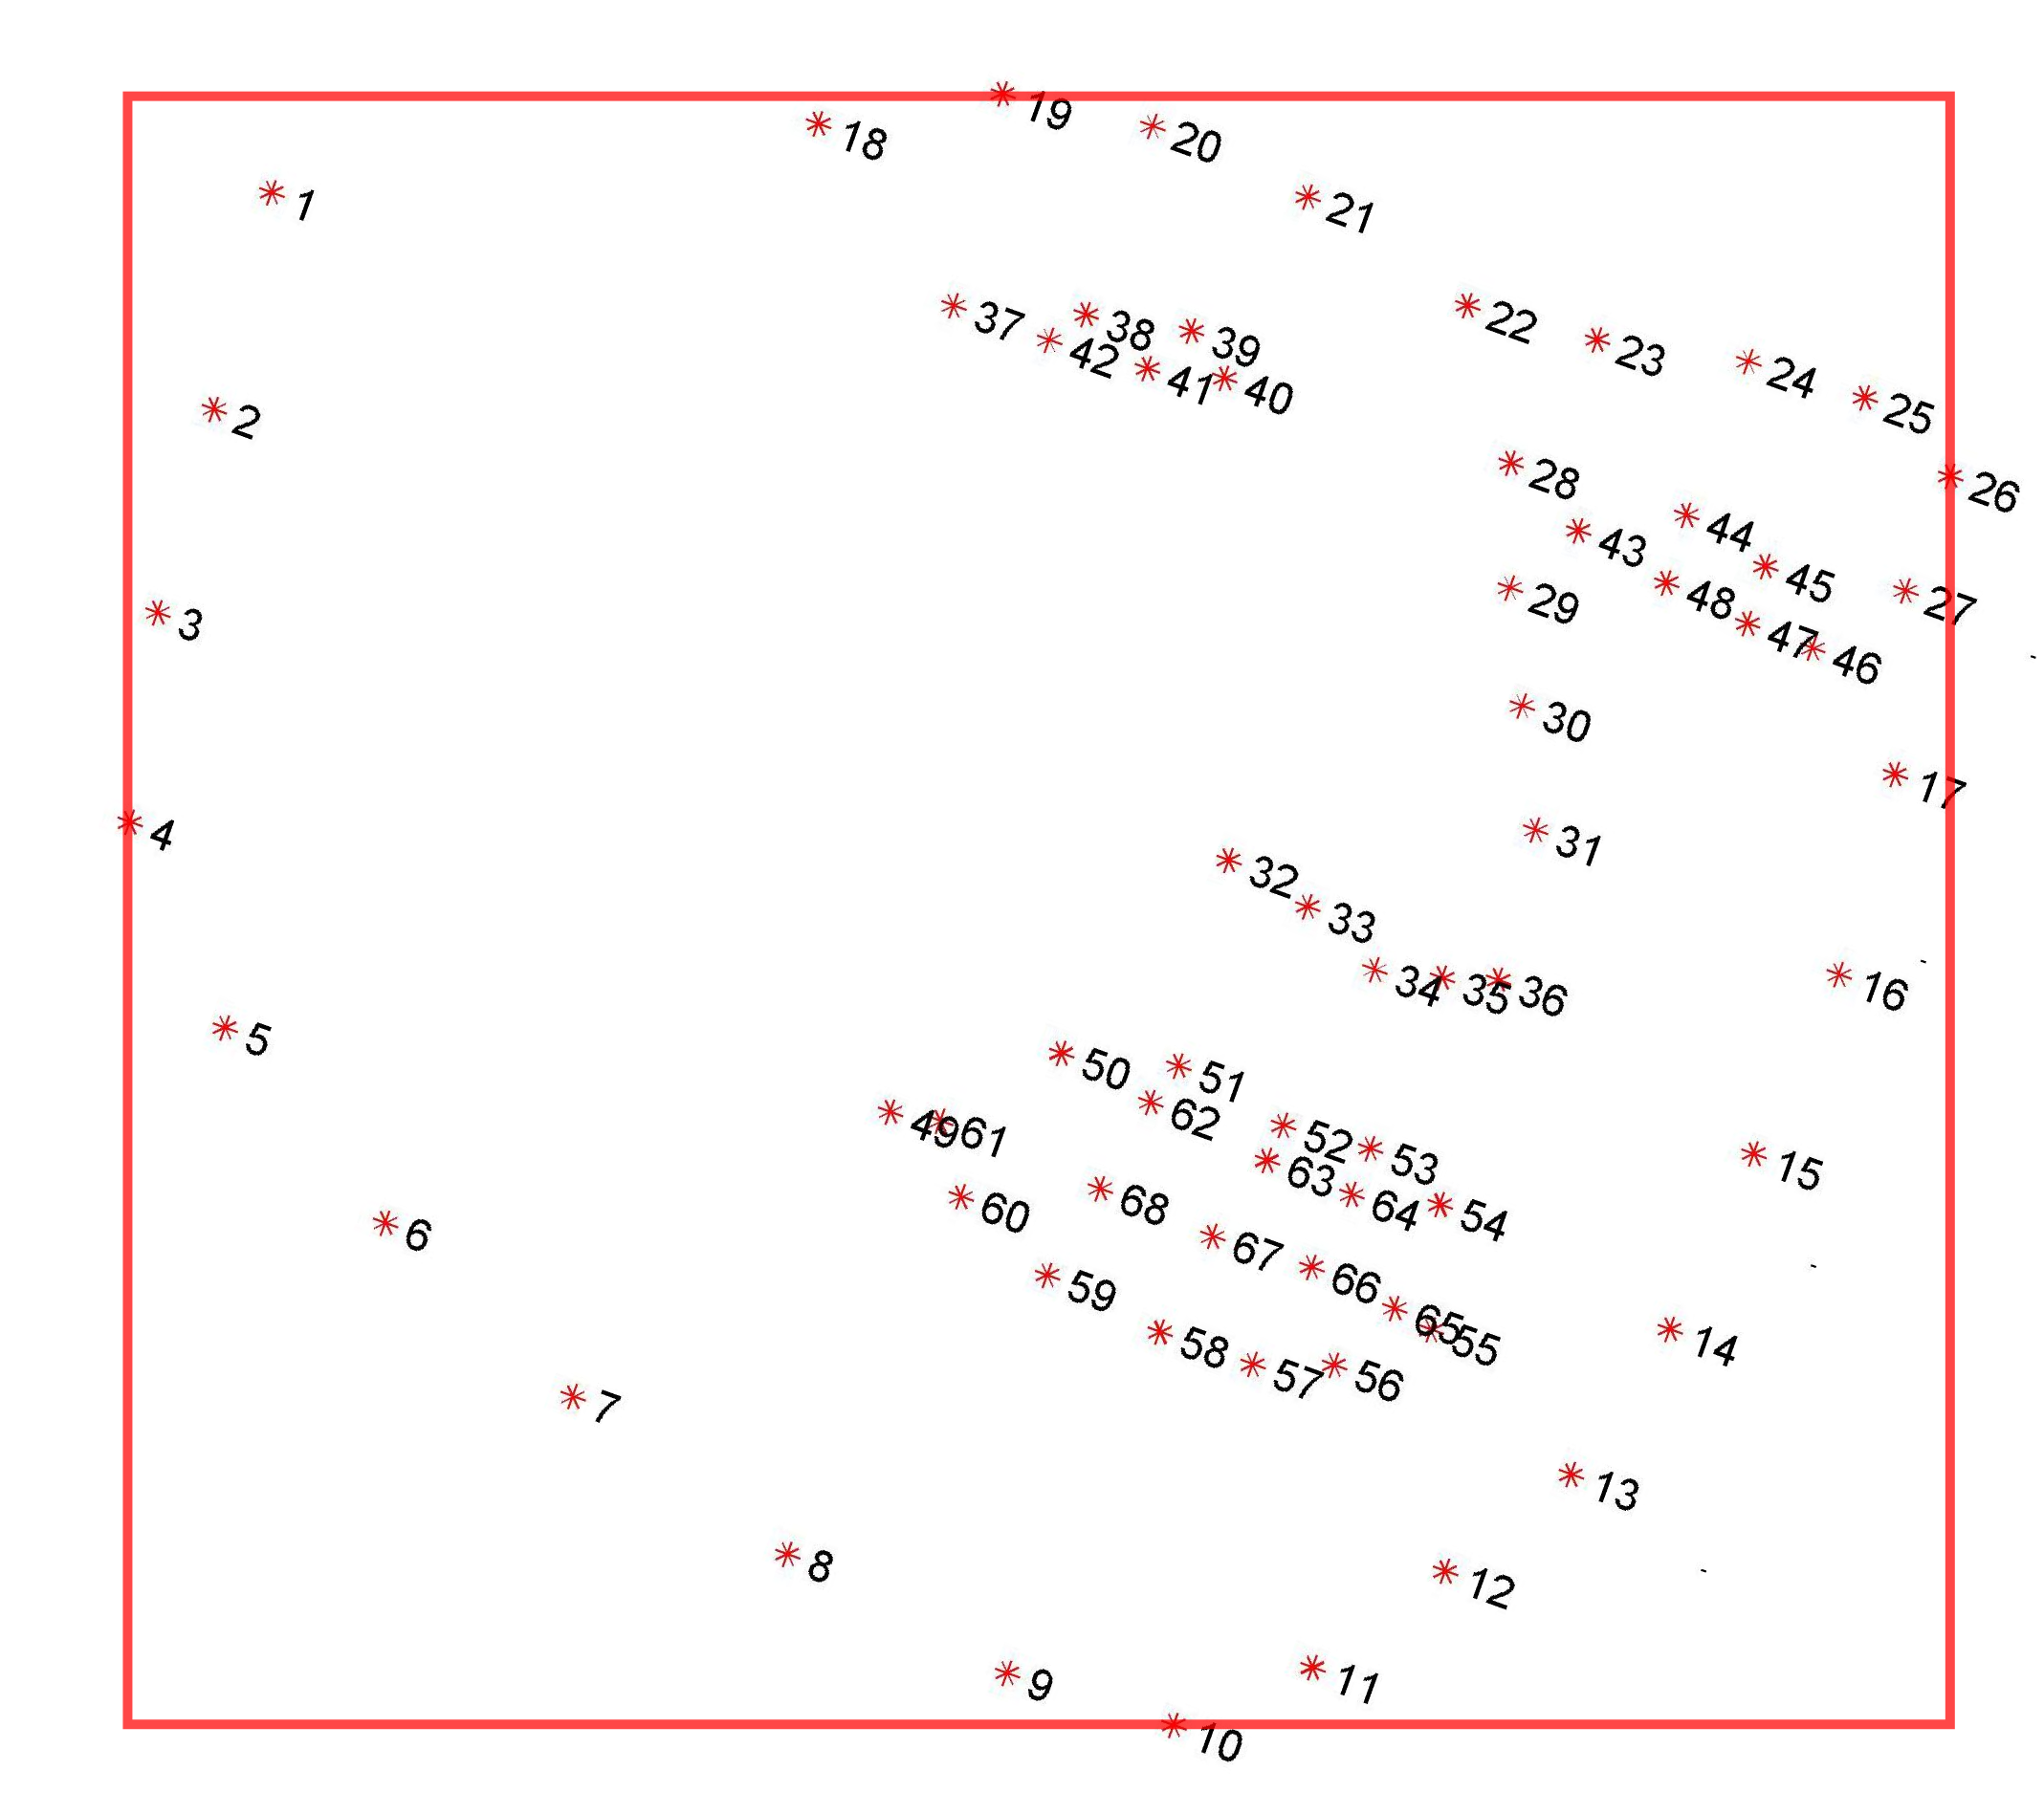
\includegraphics[width=\textwidth/2 - 10pt]{facial_landmarks_2.png}
    
    \caption{Facial landmarks\\Source: \href{https://ibug.doc.ic.ac.uk/resources/300-W/}{ibug}}
    \label{}
\end{figure}